\documentclass[11pt,a4paper]{article}
%%%%%%%%%%%%%%%%%%%%%%%%% Credit %%%%%%%%%%%%%%%%%%%%%%%%

% template ini dibuat oleh martin.manullang@if.itera.ac.id untuk dipergunakan oleh seluruh sivitas akademik itera.

%%%%%%%%%%%%%%%%%%%%%%%%% PACKAGE starts HERE %%%%%%%%%%%%%%%%%%%%%%%%
\usepackage{graphicx}
\usepackage{caption}
\usepackage[expansion=false]{microtype}
\captionsetup[table]{name=Tabel}
\captionsetup[figure]{name=Gambar}
\usepackage{tabulary}
\usepackage{minted}
% \usepackage{amsmath}
\usepackage{fancyhdr}
% \usepackage{amssymb}
% \usepackage{amsthm}
\usepackage{placeins}
% \usepackage{amsfonts}
\usepackage{graphicx}
\usepackage[all]{xy}
\usepackage{tikz}
\usepackage{verbatim}
\usepackage[left=2cm,right=2cm,top=3cm,bottom=2.5cm]{geometry}
\usepackage{hyperref}
\hypersetup{
    colorlinks,
    linkcolor={red!50!black},
    citecolor={blue!50!black},
    urlcolor={blue!80!black}
}
\usepackage{caption}
\usepackage{subcaption}
\usepackage{multirow}
\usepackage{psfrag}
\usepackage[T1]{fontenc}
\usepackage[scaled]{beramono}
% Enable inserting code into the document
\usepackage{listings}
\usepackage{xcolor} 
% custom color & style for listing
\definecolor{codegreen}{rgb}{0,0.6,0}
\definecolor{codegray}{rgb}{0.5,0.5,0.5}
\definecolor{codepurple}{rgb}{0.58,0,0.82}
\definecolor{backcolour}{rgb}{0.95,0.95,0.92}
\definecolor{LightGray}{gray}{0.9}
\lstdefinestyle{mystyle}{
backgroundcolor=\color{backcolour},   
commentstyle=\color{green},
keywordstyle=\color{codegreen},
numberstyle=\tiny\color{codegray},
stringstyle=\color{codepurple},
basicstyle=\ttfamily\footnotesize,
breakatwhitespace=false,         
breaklines=true,                 
captionpos=b,                    
keepspaces=true,                 
numbers=left,                    
numbersep=5pt,                  
showspaces=false,                
showstringspaces=false,
showtabs=false,                  
tabsize=2
}
\lstset{style=mystyle}
\renewcommand{\lstlistingname}{Kode}
%%%%%%%%%%%%%%%%%%%%%%%%% PACKAGE ends HERE %%%%%%%%%%%%%%%%%%%%%%%%


%%%%%%%%%%%%%%%%%%%%%%%%% Data Diri %%%%%%%%%%%%%%%%%%%%%%%%
\newcommand{\studentlist}{
    \item \textbf{Joshua Palti Sinaga (122140141)}
    \item \textbf{Rustian Afencius Marbun (122140155)}
}
\newcommand{\course}{\textbf{Pembelajaran Mendalam (IF25-40401)}}
\newcommand{\assignment}{\textbf{Tugas Eksplorasi}}

%%%%%%%%%%%%%%%%%%% using theorem style %%%%%%%%%%%%%%%%%%%%
\newtheorem{thm}{Theorem}
\newtheorem{lem}[thm]{Lemma}
\newtheorem{defn}[thm]{Definition}
\newtheorem{exa}[thm]{Example}
\newtheorem{rem}[thm]{Remark}
\newtheorem{coro}[thm]{Corollary}
\newtheorem{quest}{Question}[section]
%%%%%%%%%%%%%%%%%%%%%%%%%%%%%%%%%%%%%%%%
\usepackage{lipsum}%% a garbage package you don't need except to create examples.
\pagestyle{fancy}
\lhead{Joshua Palti Sinaga (122140141), Rustian Afencius Marbun (122140155)}
\rhead{ \thepage}
\cfoot{\textbf{Tugas Eksplorasi: Eksperimen Arsitektur ResNet-34}}
\renewcommand{\headrulewidth}{0.4pt}
\renewcommand{\footrulewidth}{0.4pt}

%%%%%%%%%%%%%%  Shortcut for usual set of numbers  %%%%%%%%%%%

\newcommand{\N}{\mathbb{N}}
\newcommand{\Z}{\mathbb{Z}}
\newcommand{\Q}{\mathbb{Q}}
\newcommand{\R}{\mathbb{R}}
\newcommand{\C}{\mathbb{C}}
\setlength\headheight{14pt}

%%%%%%%%%%%%%%%%%%%%%%%%%%%%%%%%%%%%%%%%%%%%%%%%%%%%%%%555
\begin{document}
\thispagestyle{empty}
\begin{center}

\includegraphics[scale = 0.15]{Figure/ifitera-header.png}
\vspace{0.1cm}
\end{center}
\noindent
\rule{17cm}{0.2cm}\\[0.3cm]
Mata Kuliah: \course \hfill Tugas: \assignment\\[0.1cm]
{Kelompok NgodingDiKertas:} \hfill Tanggal: \textbf{29 September 2025}
\begin{enumerate}
    \studentlist
\end{enumerate}
\rule{17cm}{0.05cm}
\vspace{0.1cm}



%%%%%%%%%%%%%%%%%%%%%%%%%%%%%%%%%%%%%%%%%%%%% BODY DOCUMENT %%%%%%%%%%%%%%%%%%%%%%%%%%%%%%%%%%%%%%%%%%%%%

\begin{center}
\section*{Eksperimen Arsitektur ResNet-34}
\end{center}
\vspace{0.5cm}
\section{Tahap 1: Analisis Performa Model Dasar (Plain Network)}
\subsection{Arsitektur Plain-34}
Plain-34 adalah arsitektur yang mirip dengan ResNet-34 tanpa skip connection, memiliki 34 layer untuk memproses gambar 224x224 pixels. Arsitektur dimulai dengan convolutional layer 7x7 (stride 2, 64 channel), batch normalization, ReLU, dan max pooling 3x3 (stride 2). Kemudian terdapat empat stage: Stage 1 (3 block, 64 channel), Stage 2 (4 block, 128 channel), Stage 3 (6 block, 256 channel), dan Stage 4 (3 block, 512 channel), dengan stride 2 pada block pertama di stage 2-4. Setiap Plain Block terdiri dari dua layer Conv 3x3 + BatchNorm + ReLU. Arsitektur diakhiri dengan global average pooling dan fully connected layer untuk 5 kelas. Perbedaan utama dengan ResNet-34 adalah output block langsung diproses tanpa dijumlahkan dengan input (tidak ada skip connection).

\subsection{Konfigurasi Pelatihan}
Konfigurasi pelatihan untuk Plain-34 menggunakan learning rate 0.001 (1e-3) dengan optimizer SGD. Batch size untuk training adalah 32, sedangkan untuk validation adalah 64. Model dilatih selama 8 epoch menggunakan CrossEntropyLoss sebagai loss function.

\subsection{Implementasi}
Implementasi menggunakan PyTorch dengan PlainBlock yang terdiri dari dua Conv3x3-BN-ReLU secara berurutan tanpa skip connection. Dataset 5 kelas makanan Indonesia dibagi 80\% training dan 20\% validation. Model dilatih 8 epoch dengan monitoring loss dan accuracy.

\subsection{Hasil Pelatihan}
Hasil menunjukkan performa rendah dengan 21.29M parameter. Training loss turun konsisten (1.609→1.591), validation loss stabil di ~1.57. Akurasi sangat rendah: training 22.7\%, validation 24.7\%, best validation 27.1\% (epoch 5), hanya sedikit di atas random guessing (20\%). Overfitting monitor menunjukkan nilai negatif setelah epoch 2, mengindikasikan model menghafal training data tanpa generalisasi baik.
\begin{figure}[h]
\centering
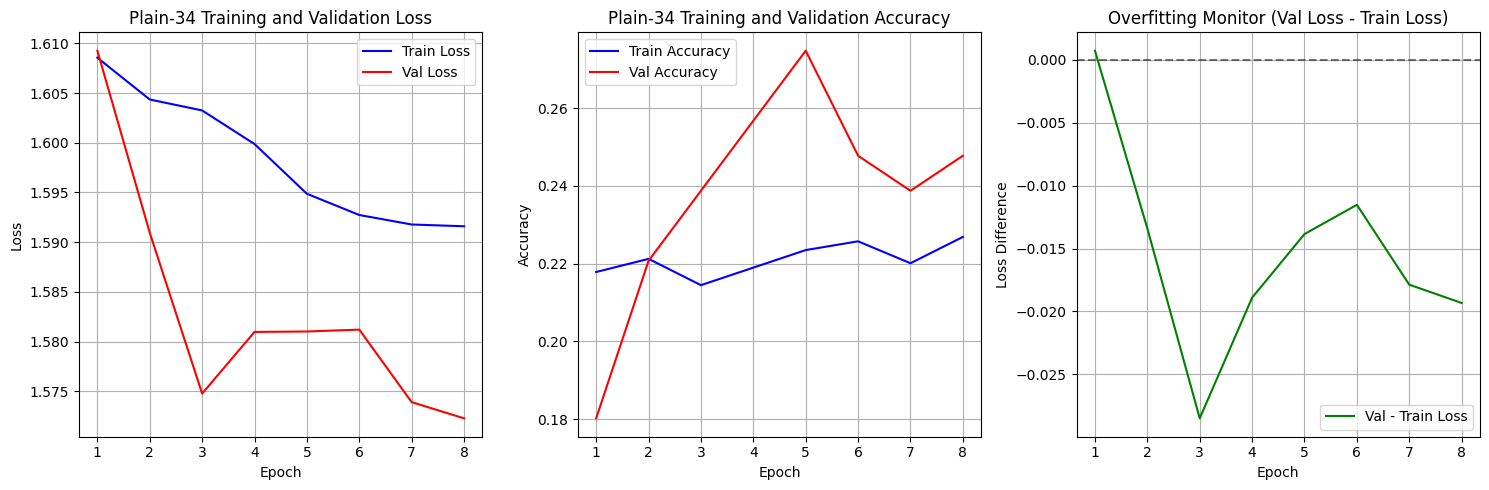
\includegraphics[width=0.75\textwidth]{Figure/plainnet34.png}
\caption{Grafik Training dan Validation Plain-34}
\label{fig:plain34}
\end{figure}

\subsection{Analisis}
Performa Plain-34 sangat rendah (max 27\%) menunjukkan masalah degradasi pada jaringan dalam tanpa skip connection. 
Dengan 34 layer, gradient mengalami vanishing gradient problem karena perkalian berulang dengan nilai kecil saat backpropagation, 
menyebabkan layer awal tidak ter-update efektif. Overfitting terlihat dari validation loss lebih rendah dari training loss setelah epoch 2, 
dan validation accuracy turun setelah puncak di epoch 5.

\section{Tahap 2: Implementasi Residual Connection (ResNet-34)}
\subsection{Modifikasi Arsitektur}
ResNet-34 identik dengan Plain-34 namun menambahkan skip connection pada setiap block. Perbedaan kunci: Plain-34 
menggunakan output = ReLU(Conv2(ReLU(Conv1(x)))), sedangkan ResNet-34 menggunakan output = ReLU(Conv2(ReLU(Conv1(x))) + x). 
Penambahan input x (skip connection) menciptakan "jalan pintas" untuk aliran gradient. Residual block menyimpan input sebagai identity, 
memproses melalui Conv-BN-ReLU-Conv-BN menghasilkan F(x), lalu menjumlahkan F(x) + x sebelum ReLU final. Model hanya perlu belajar residual F(x) = H(x) - x, 
bukan transformasi penuh H(x). Untuk dimensi berbeda, digunakan downsample layer (Conv 1x1). Semua konfigurasi lain sama dengan Plain-34 untuk perbandingan yang adil.

\subsection{Implementasi}
Implementasi ResNetBlock memodifikasi forward function dengan menyimpan input sebagai identity, memproses melalui Conv-BN-ReLU-Conv-BN, lalu menjumlahkan hasil dengan identity (skip connection: out + identity) sebelum ReLU final. Downsample digunakan jika dimensi berbeda.

\subsection{Hasil Pelatihan}
ResNet-34 menunjukkan peningkatan signifikan dengan parameter sama (21.29M). Loss turun smooth: training 1.605→1.538, validation 1.605→1.516. Akurasi meningkat drastis: training 34.4\%, validation 30.0\%, best validation 44.7\% (epoch 6), jauh melampaui Plain-34. Learning curve konsisten naik hingga epoch 6. Overfitting lebih terkontrol dengan loss difference stabil, menunjukkan skip connection membantu regularisasi implisit.
\begin{figure}[h]
\centering
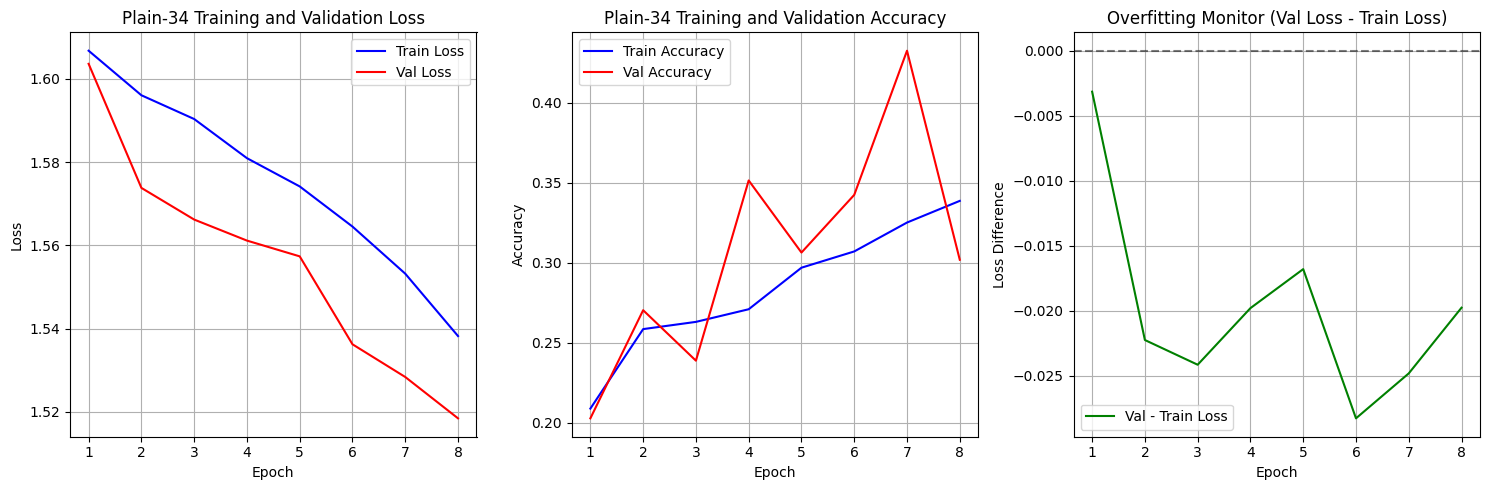
\includegraphics[width=0.65\textwidth]{Figure/resnet34.png}
\caption{Grafik Training dan Validation ResNet-34}
\label{fig:resnet34}
\end{figure}

\subsection{Perbandingan dengan Plain-34}

Skip connection memberikan dampak signifikan. Best validation accuracy meningkat dari 27.1\%→44.7\%, final validation accuracy +5.3\%, training accuracy +11.7\%. Loss turun: validation -0.057, training -0.053. Yang penting, peningkatan ini dicapai dengan parameter sama persis (21.29M), membuktikan efektivitas murni dari skip connection. ResNet-34 menunjukkan konvergensi lebih cepat, kurva smooth dan stabil, berbeda dengan Plain-34 yang stagnan dan fluktuatif.

\section{Tahap 3: Eksperimen Modifikasi Arsitektur ResNet-34}
\subsection{Pemilihan Modifikasi}
Kami memilih dua modifikasi pada arsitektur ResNet-34, yaitu penggantian optimizer Adam ke AdamW dengan weight decay 5e-4, dan arsitektur ResNeXt.

\subsection{Justifikasi Pemilihan}
AdamW dipilih berdasarkan penelitian Loshchilov dan Hutter~\cite{loshchilov2017decoupled} yang membuktikan generalisasi lebih baik dari Adam melalui pemisahan weight decay dari gradient update. Weight decay 5e-4 memberikan regularisasi efektif tanpa menghambat pembelajaran.

\begin{figure}[h]
\centering
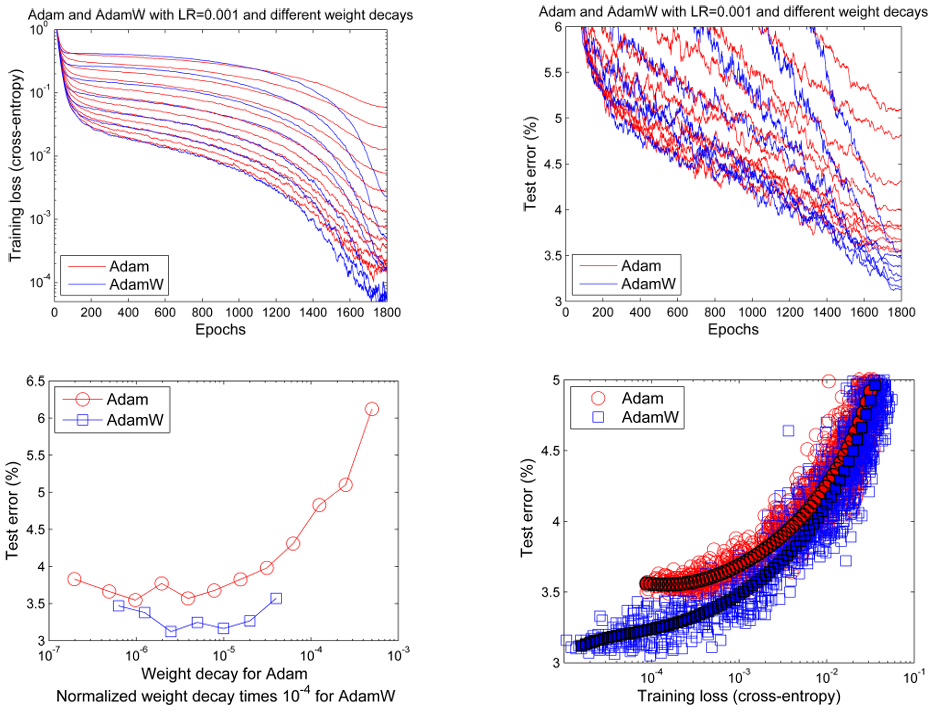
\includegraphics[width=0.5\textwidth]{Figure/tahap-3-adamw-comparison.png}
\caption{Perbandingan Adam vs AdamW (Sumber: Loshchilov \& Hutter~\cite{loshchilov2017decoupled})}
\label{fig:adamw}
\end{figure}

ResNeXt dipilih berdasarkan paper Xie et al.~\cite{xie2017aggregated} yang memperkenalkan cardinality sebagai dimensi baru. Grouped convolution membagi channel menjadi kelompok independen, meningkatkan kapasitas model tanpa menambah parameter signifikan. Cardinality 16 dipilih berdasarkan rekomendasi paper untuk keseimbangan optimal.

\subsection{Modifikasi 1: Optimizer AdamW}
\subsubsection{Implementasi}
Optimizer diubah dari Adam ke AdamW (weight decay 5e-4) dengan learning rate 3e-4, batch size 32/64, dan 8 epoch. AdamW memisahkan weight decay dari gradient update, berbeda dengan L2 regularization pada Adam standar.

\subsubsection{Hasil Pelatihan}
Best validation accuracy 82.88\%, meningkat 38.2 poin dari baseline (44.7\%). Metrik F1 0.8245, precision 0.8410, recall 0.8288 menunjukkan performa seimbang. Konvergensi smooth dengan overfitting terkontrol membuktikan efektivitas weight decay sebagai regularisasi.

\begin{figure}[h]
\centering
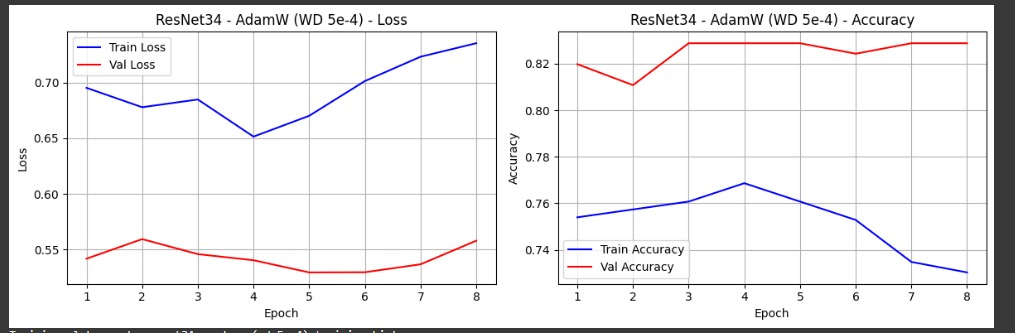
\includegraphics[width=0.55\textwidth]{Figure/tahap-3-resnet34-adamw.jpg}
\caption{Grafik Training dan Validation ResNet-34 dengan AdamW}
\label{fig:resnet34-adamw}
\end{figure}

\subsubsection{Analisis}
Peningkatan dari 44.7\%→82.88\% membuktikan dampak pemisahan weight decay dari gradient update. AdamW mencegah weight decay tereduksi oleh adaptive learning rate, menghasilkan regularisasi lebih efektif dan optimisasi lebih stabil.

\subsection{Modifikasi 2: Arsitektur ResNeXt-like Block}
\subsubsection{Implementasi}
ResNet block diganti dengan ResNeXt-like block (grouped convolution, cardinality 16). Input dibagi 16 kelompok independen, diproses Conv 3x3, lalu diagregat sebelum skip connection. Diuji dengan Adam (LR 1e-3) dan AdamW (LR 1e-3, WD 5e-4), batch size 32/64, 8 epoch.

\subsubsection{Hasil Pelatihan}
ResNeXt+Adam: 86.94\% accuracy (+42.2 poin), F1 0.8684, precision 0.8858, recall 0.8694. ResNeXt+AdamW (terbaik): 94.14\% accuracy, F1 0.9428, precision 0.9509, recall 0.9414. 

\begin{figure}[h]
\centering
\begin{subfigure}{0.49\textwidth}
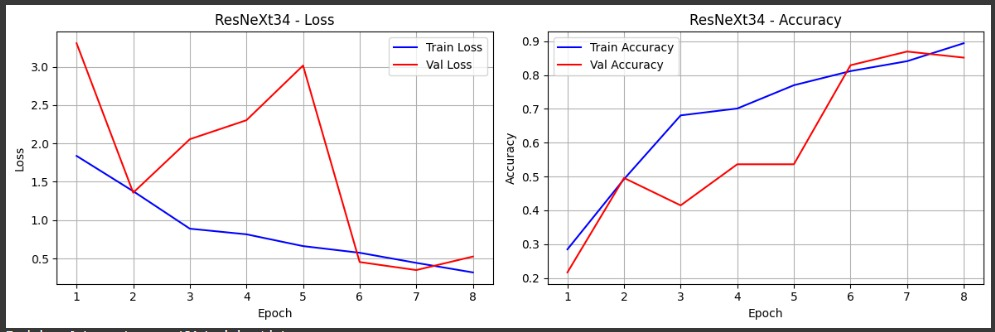
\includegraphics[width=\textwidth]{Figure/tahap-3-resnext34.jpg}
\caption{ResNeXt34 dengan Adam}
\label{fig:resnext34-adam}
\end{subfigure}
\hfill
\begin{subfigure}{0.49\textwidth}
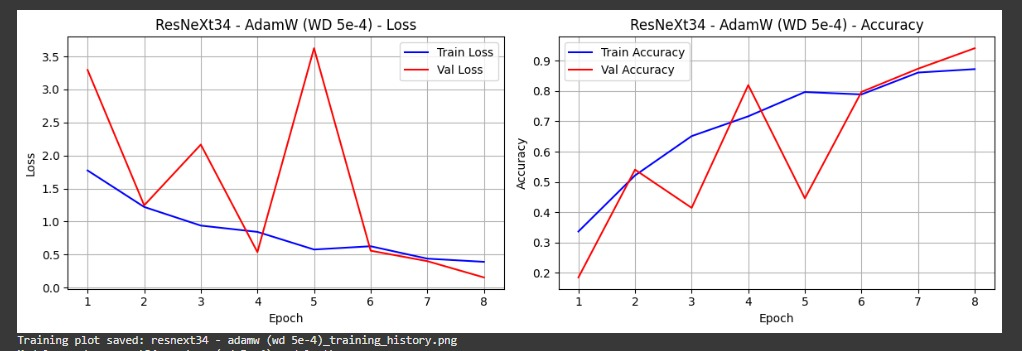
\includegraphics[width=\textwidth]{Figure/tahap-3-resnext34-adamw.jpg}
\caption{ResNeXt34 dengan AdamW}
\label{fig:resnext34-adamw}
\end{subfigure}
\caption{Perbandingan Grafik Training ResNeXt34}
\label{fig:resnext34-comparison}
\end{figure}

\subsubsection{Analisis}
Grouped convolution (16 jalur paralel) meningkatkan kapasitas representasi melalui ekstraksi fitur lebih beragam. Peningkatan dari 44.7\%→86.94\% membuktikan efektivitas arsitektur. Kombinasi ResNeXt+AdamW (94.14\%) menunjukkan sinergi optimal, konsisten dengan temuan Xie et al.~\cite{xie2017aggregated}.

\subsection{Perbandingan Modifikasi}
\subsubsection{ResNet-34: Adam vs AdamW}
Penggantian Adam ke AdamW meningkatkan akurasi 38.2 poin (hampir 2x lipat). Peningkatan recall > precision menunjukkan identifikasi kelas lebih baik, memvalidasi temuan paper~\cite{loshchilov2017decoupled} tentang pentingnya pemisahan weight decay.
\begin{table}[h]
\centering
\caption{Perbandingan ResNet-34 dengan Adam vs AdamW}
\begin{tabular}{|l|c|c|c|}
\hline
\textbf{Metrik} & \textbf{Adam} & \textbf{AdamW} & \textbf{Peningkatan} \\ \hline
Best Val Accuracy & 44.7\% & 82.88\% & +38.2\% \\ \hline
F1 Score & 0.7129 & 0.8245 & +0.1116 \\ \hline
Precision & 0.7947 & 0.8410 & +0.0463 \\ \hline
Recall & 0.7297 & 0.8288 & +0.0991 \\ \hline
\end{tabular}
\end{table}

\subsubsection{ResNeXt-34: Adam vs AdamW}
AdamW meningkatkan akurasi 7.2 poin (86.94\%→94.14\%), membuktikan efektivitas untuk berbagai arsitektur. Peningkatan seimbang precision dan recall menunjukkan generalisasi lebih baik.
\begin{table}[h]
\centering
\caption{Perbandingan ResNeXt-34 dengan Adam vs AdamW}
\begin{tabular}{|l|c|c|c|}
\hline
\textbf{Metrik} & \textbf{Adam} & \textbf{AdamW} & \textbf{Peningkatan} \\ \hline
Best Val Accuracy & 86.94\% & 94.14\% & +7.2\% \\ \hline
F1 Score & 0.8684 & 0.9428 & +0.0744 \\ \hline
Precision & 0.8858 & 0.9509 & +0.0651 \\ \hline
Recall & 0.8694 & 0.9414 & +0.0720 \\ \hline
\end{tabular}
\end{table}

\subsubsection{Dampak Arsitektur ResNet vs ResNeXt (Optimizer Sama)}
Dengan optimizer sama (Adam), ResNeXt mengungguli ResNet 42.2 poin (hampir 2x lipat). Peningkatan recall lebih besar membuktikan grouped convolution menangkap variasi kelas lebih efektif, konsisten dengan paper~\cite{xie2017aggregated}.

\section{Peran dan Kontribusi AI Assistant}

Dalam pengerjaan tugas ini, AI Assistant (Google Gemini dan ChatGPT) digunakan untuk membantu 
implementasi kode dan \textit{brainstorming} terkait resnet34 dan modifikasi yang akan kami lakukan. 
Untuk detail lengkap prompt dan interaksi dengan AI, dapat dilihat pada link berikut: (1) Google Gemini: \url{https://g.co/gemini/share/3c7328db60e2}, 
dan (2) ChatGPT: \url{https://chatgpt.com/share/68dfb201-d978-8001-b60b-7f91d1ee34a5}.

\newpage
\bibliographystyle{IEEEtran}
\bibliography{Referensi}
\end{document}
